\section{Phase selection and intermittency of exciton-polariton condensates in 1D periodic structures}\label{Ch3}
%\subsection{Background}
Since the discovery of the superfluid--Mott insulator transition with cold atoms in optical lattices~\cite{Jaksch:1998aa,Greiner:2002aa}, systems with bosons in periodic potentials have drawn much attention for both fundamental and applied interests.
% While the cold atoms in periodic optical lattices are probably the cleanest system, they have extremely low critical temperature to form the condensation due to heavy atomic masses.
Compared to the cold atoms, exciton-polaritons in semiconductor microcavities~\cite{Weisbuch:1992aa,Deng:2002aa,Kavokin:2005kj} possess substantially smaller effective masses and can condense not only at liquid helium~\cite{Kasprzak:2006aa,Balili:2007aa,Lai:2007aa} but also up to room temperature~\cite{Baumberg:2008aa,Lerario:2017aa}.
This advantage makes polaritons in artificial periodic potentials an excellent alternative platform for studying many-body physics, gap solitons~\cite{Tanese:2013aa,Buller:2016aa}, topological polariton states~\cite{Karzig:2015aa,Gulevich:2016aa}, and classical~\cite{Ohadi:2017aa} and quantum~\cite{Liew:2018aa} simulators.

% The physics of polariton condensation is quite different from traditional cold atoms.
There is a significant difference between polariton BEC and traditional BEC.
In the former, external pumping (coherent or incoherent) is required to create and maintain polaritons due to their finite lifetime in the microcavity, and this pumping usually prohibits the particles from reaching thermal equilibrium, so that steady-state condensates can be formed in excited states with many-body correlations.
% Particularly, for polariton condensates in periodic potentials, the condensation at the edges of the Brillouin zone, namely $\pi$-condensation in one-dimensional (1D) lattices~\cite{Lai:2007aa} and $p$- and $d$-condensation in two-dimensional (2D) lattices~\cite{Kim:2011aa}, as well as the mixed condensates~\cite{Zhang:2015aa} have been observed.
Particularly, for polariton BEC in periodic potentials, several non-trivial condensations have been reported, for example $\pi$-condensation in 1D lattices~\cite{Lai:2007aa} and $p$- and $d$-condensation in 2D lattices~\cite{Kim:2011aa}, as well as mixed condensates~\cite{Zhang:2015aa}.

% Loading cavity photons and quantum-well excitons into separate periodic potentials, one can achieve multivalley (instead of $\pi$- or $0$-) condensation~\cite{Sun:2017ab}.
Moreover, polariton condensation in the presence of distributed gain and loss for the single-particle states is expected to be accompanied by the formation of spontaneous currents~\cite{Nalitov:2017aa}.
Another recent finding is polariton condensation in flat bands of 1D~\cite{Baboux:2016aa} and 2D~\cite{Klembt:2017aa,Whittaker:2018ab,Sun:2018aa} periodic systems.
Such condensates provide a strong enhancement of the effects of polariton--polariton interaction due to the reduced kinetic energy of the particles.

In this chapter, we consider a 1D polariton system in a complex periodic potential and complex nonlinearity to account for polariton--polariton interaction and gain saturation.
We show that for a detailed description of the system, it is necessary to consider the imaginary part of the periodic potential, which describes the distributed gain and losses~\cite{Winkler:2016aa} of the single-particle states in the microcavity.
By carefully tuning the parameters of the complex potential (such as the height and width of its imaginary part), one can control the state of the system and demonstrate that several conceptually different situations are possible.

In the case of a relatively large bandwidth (i.e., a large energy difference between the $0$- and $\pi$-states for the single-particle spectrum), we find that the condensation changes from $0$-state to $\pi$-state (or vice versa) with increasing interaction between the particles.
This counter-intuitive effect takes place since the state with maximal gain becomes unstable due to the strongly interacting particles, while the state with minimal gain starts to accumulate bosons.
Consequently, the total number of particles in the condensate is not maximized.

% The crossover from 0- to $\pi$-condensate (or vice versa) happens by formation of propagating dark solitons, which is another surprising result.
Another interesting result is the formation of propagating dark solitons when the crossover between $0$- and $\pi$-state condensates happens.
At a certain magnitude of polariton--polariton interaction, comparable with the bandwidth, and as a result of soliton propagation, the polaritons are distributed quasi-homogeneously along the dispersion curve instead of accumulating in a single quantum state as in typical condensation.
In this case, the polaritons occupy the band more or less uniformly, and short correlations in space and time manifest as intermittency of the condensate state.

% The paper is organized as follows. In Section II below we introduce the generalized Ginzburg-Landau model to describe the exciton-polariton condensate in 1D complex-valued periodic potentials and give a brief description of the cases we will focus in our numerical simulations. In Section III, the simulation results are presented and discussed, and Section IV contains conclusions.

%
% ------------------------------------------------------
%
\subsection{Theoretical model}
We study the solutions to the 1D generalized Ginzburg--Landau equation (GLE)~\cite{Keeling:2008js},
\begin{equation}\label{eq:CH4_GPeq}
    \mi\hbar\partial_t\psi =
    -\frac{\hbar^2}{2 m^*}\partial^2_x\psi + V\left(x\right)\psi
    +\left(\alpha-\mi\beta\right)|\psi|^2\psi,
\end{equation}
where $\psi\left(x,t\right)$ is the wave function of polariton condensate, $V(x)=V(x+a)$ is the complex periodic potential with the lattice constant $a$, $m^*$ is the polariton effective mass, $\alpha$ is the polariton--polariton interaction constant~\cite{Ciuti:1998aa,Tassone:1999aa,Magnusson:2011aa}, and $\beta>0$ accounts for the gain-saturated nonlinearity of the system~\cite{Keeling:2008js, Karpov:2015aa}.
By scaling the wave function $\psi\rightarrow\psi/\sqrt{\beta}$, one can set $\beta=1$ to obtain the dimensionless interaction constant $\alpha/\beta$.
To get Eq.~\eqref{eq:CH4_GPeq}, one can consider the steady-state condition of Eq.~\eqref{eq:Ch1_inchoerent_pumping2} and substitute the result into Eq.~\eqref{eq:Ch1_inchoerent_pumping1}
\begin{eqnarray}
    \label{eq:CH4_GPEQ1}
\mi\hbar \frac{\partial}{\partial t} \psi\left(\mathbf{r},t\right) &=& \left[ -\frac{\hbar^2}{2m}\nabla^2 + V\left(\mathbf{r}\right) + \alpha \abs{\psi\left(\mathbf{r},t\right)}^2 -\frac{\mi \gamma}{2} \right] \psi\left(\mathbf{r},t\right)\nonumber
    \\ &+& \frac{\mi}{2}R\frac{I\left(\mathbf{r},t\right)}{R \abs{\psi\left(\mathbf{r},t\right)}^2 + \gamma_R} \psi\left(\mathbf{r},t\right).
\end{eqnarray}
Then by expanding the last term to the first order in the limit $\frac{\gamma_R}{R\abs{\psi}^2}\gg 1$, one can get
\begin{eqnarray}
    \label{eq:CH4_GPEQ2}
\mi\hbar \frac{\partial}{\partial t} \psi\left(\mathbf{r},t\right) &=& \left[ -\frac{\hbar^2}{2m}\nabla^2 + V\left(\mathbf{r}\right) + \alpha \abs{\psi\left(\mathbf{r},t\right)}^2 -\frac{\mi \gamma}{2} \right] \psi\left(\mathbf{r},t\right)\nonumber
    \\ &+& \frac{\mi}{2}R I\left(\mathbf{r},t\right)\gamma_R\psi\left(\mathbf{r},t\right) -\frac{\mi R^2}{2\gamma_R}\abs{\psi\left(\mathbf{r},t\right)}^2\psi\left(\mathbf{r},t\right).
\end{eqnarray}
In Eq.~\eqref{eq:CH4_GPeq}, the potential is complexed value, by comparing with Eq.~\eqref{eq:CH4_GPEQ2}, we have
\begin{equation}
    \textrm{Re}\left[ V\left(x\right)\right] = V\left(\mathbf{r}\right),~ ~ ~ \textrm{Im}\left[V\left(x\right)\right]= -\frac{1}{2}\left( \gamma - RI\left(\mathbf{r},t\right)\gamma_R \right)
\end{equation}
and similarly
\begin{equation}
    \beta = \frac{R^2}{\gamma_R}.
\end{equation}


By applying the generalized GLE~\eqref{eq:CH4_GPeq}, one has (i) a simple form, as compared to more detailed descriptions involving the incoherent exciton reservoir, and (ii) a minimal set of parameters, which allows us to obtain good qualitative insight into the physics of exciton-polariton condensation in periodic potential.
We want to note that when the system reaches a steady-state on long time scales, the interaction and dissipative parameters get rescaled by taking the reservoir steady-state into account.
However, in the general form of Eq.~\eqref{eq:CH4_GPeq}, the periodicity of the potential and the presence of the two types of non-linearities (interaction and dissipation) remain unchanged, which is a great benefit of the Ginzburg--Landau approach.
Another advantage of Eq.~\eqref{eq:CH4_GPeq} is that it can be easily compared with the complex GLE without a periodic potential, which is a well-established model for the study of nonlinear phenomena in different areas, see for example~\cite{Aranson:2002aa} for a review.

% We describe the complex potential $V(x)=V_R(x)+{\mi}V_I(x)$ as a superposition of square wells in both real and imaginary part of it, but with different widths.
To describe the complex potential $V(x)=V_R(x)+{\mi}V_I(x)$ in one unit cell ($0\le x <a$), we introduce
% Namely, within the unit cell, $0 \le x < a$, we have (see Fig.~\ref{CH4_fig:1-1}, upper panels)
%
\begin{subequations}\label{eq:CH4_CoxV}
\begin{align}
  V_R(x) &= U\,\Theta\!\left(\left | x -\frac{a}{2} \right |-\frac{a_R}{2} \right), \\
  V_I(x) &= W\,\Theta\!\left(\frac{a_I}{2}-\left | x -\frac{a}{2} \right | \right)-\Gamma,
\end{align}
\end{subequations}
%
where $\Theta(x)$ is the Heaviside step function, $U$ is the height of the potential barriers, $W$ describes the local gain from the pumping, and $\Gamma$ defines the uniform losses of the system (due to finite polariton lifetime in the microcavity).
Parameters $a_R$ and $a_I$ are the widths of the real potential wells and the imaginary potential barriers, respectively.
By varying the parameters, one can get the potential in Fig.~\ref{CH4_fig:1-1}.

Complex potential [Eq.~\eqref{eq:CH4_CoxV}] reflects the experimental situation in which the system is pumped from the excitonic reservoirs created in the barriers.
Due to exciton-polariton interaction, the particles move into the wells (similar to the case of 2D lattices of trapped polariton condensates~\cite{Ohadi:2017aa}), so that the gain part of the potential (parameter $W$) is located at the wells.
The excitonic reservoirs also increase the barrier heights.
It should be noted that a uniform microcavity subject to a periodic pumping with period $a$ is described by the same model [Eq.~\eqref{eq:CH4_CoxV}].
This pumping not only produces periodic gain (periodic imaginary part), but also periodic repulsive potential (periodic real part).
This setup has a clear benefit in that period $a$ can be tuned.
Since the gain is maximized in the potential wells, the $0$-state, which mainly resides in the wells, has bigger gain than the $\pi$-state, which mainly resides in the barriers~\cite{Lai:2007aa}.

It is important that, depending on the parameters of the potential in Eq.~\eqref{eq:CH4_CoxV}, the single-polariton spectrum can be categorized into four qualitatively different types.
We classify them as $\Lambda\Lambda$ [see Fig.~\ref{CH4_fig:1-1}(a), lower panel], VV [Fig.~\ref{CH4_fig:1-1}(b), lower panel], V$\Lambda$, and $\Lambda$V, depending on the position of the energy minimum (the real part of the eigenvalue) and the position of the gain minimum (the imaginary part of the eigenvalue) for the first band.
For example, the $\Lambda\Lambda$-type corresponds to the case when the minimum energy and minimum gain are both at the edge of the first Brillouin zone at $k=\pm \pi/a$ [see Fig.~\ref{CH4_fig:1-1}(a)].
We also define the effective widths of the bands $\Delta E_R$ and $\Delta E_I$.

%
%
%
\begin{figure}[ht]
\centering
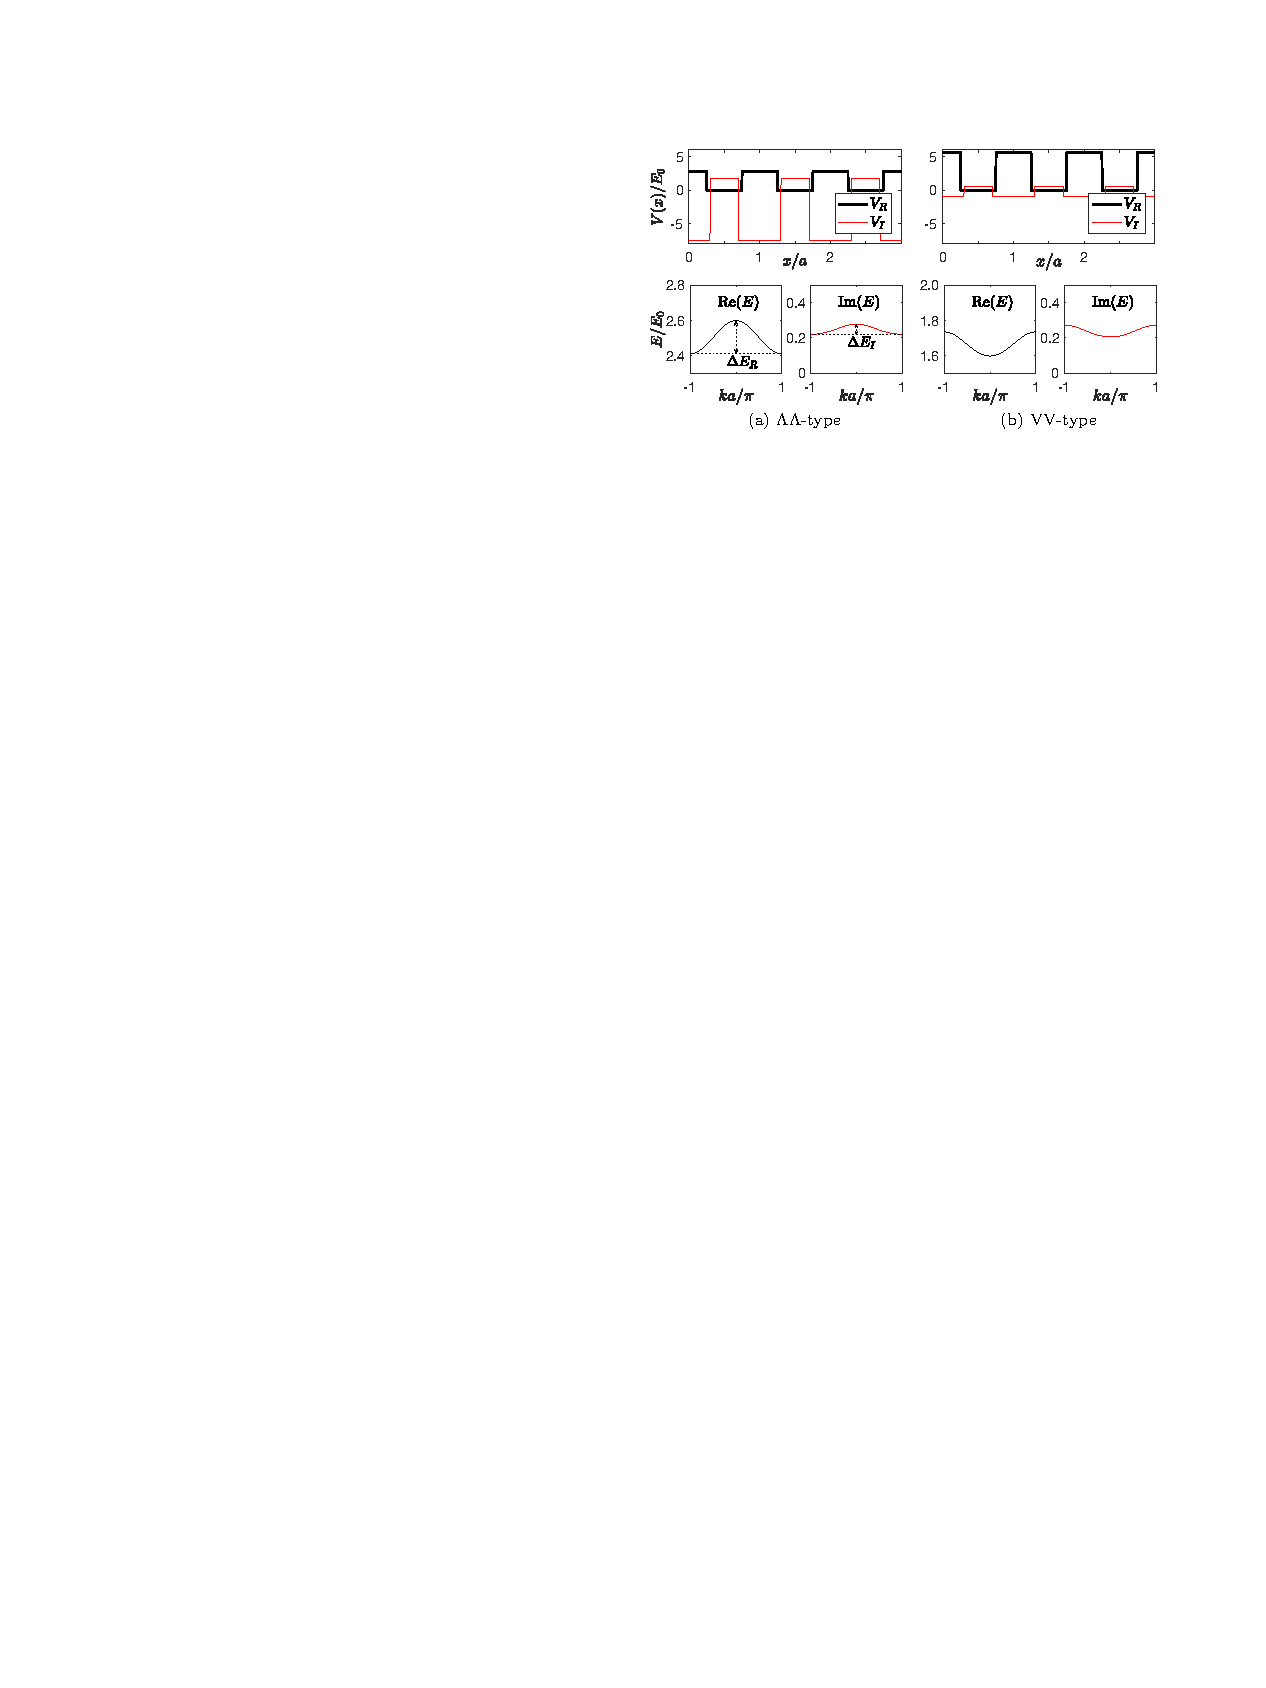
\includegraphics[width=0.75\textwidth]{Fig/Ch4/fig1.pdf}
\caption[Setup of 1D complex potentials and corresponding eigenvalues]{Complex potentials and dispersion of the first band. The real and imaginary parts are plotted with thick black lines and thin red lines, respectively. (a) The $\Lambda\Lambda$ case with the following parameters: $U = 14(\hbar^2/m^* a^2)$, $W = 3.26~U$, $\Gamma=2.64~U$. (b) The VV case with the following parameters: $U=28(\hbar^2/m^* a^2)$, $W=0.25~U$, $\Gamma= 0.16~U$. The energy bandwidth ratio ${\Delta}E_R/{\Delta}E_I \approx 3$ (a) and $2$ (b). In both cases, $a_R = 0.5a$  and $a_I = 0.4a$. The energies are measured in units of $E_0=\pi^2\hbar^2/2m^*a^2$. The figure is taken from~\cite{Yoon:2019aa}.}
\label{CH4_fig:1-1}
\end{figure}
%
%
%

\begin{figure}[!htb]
\centering
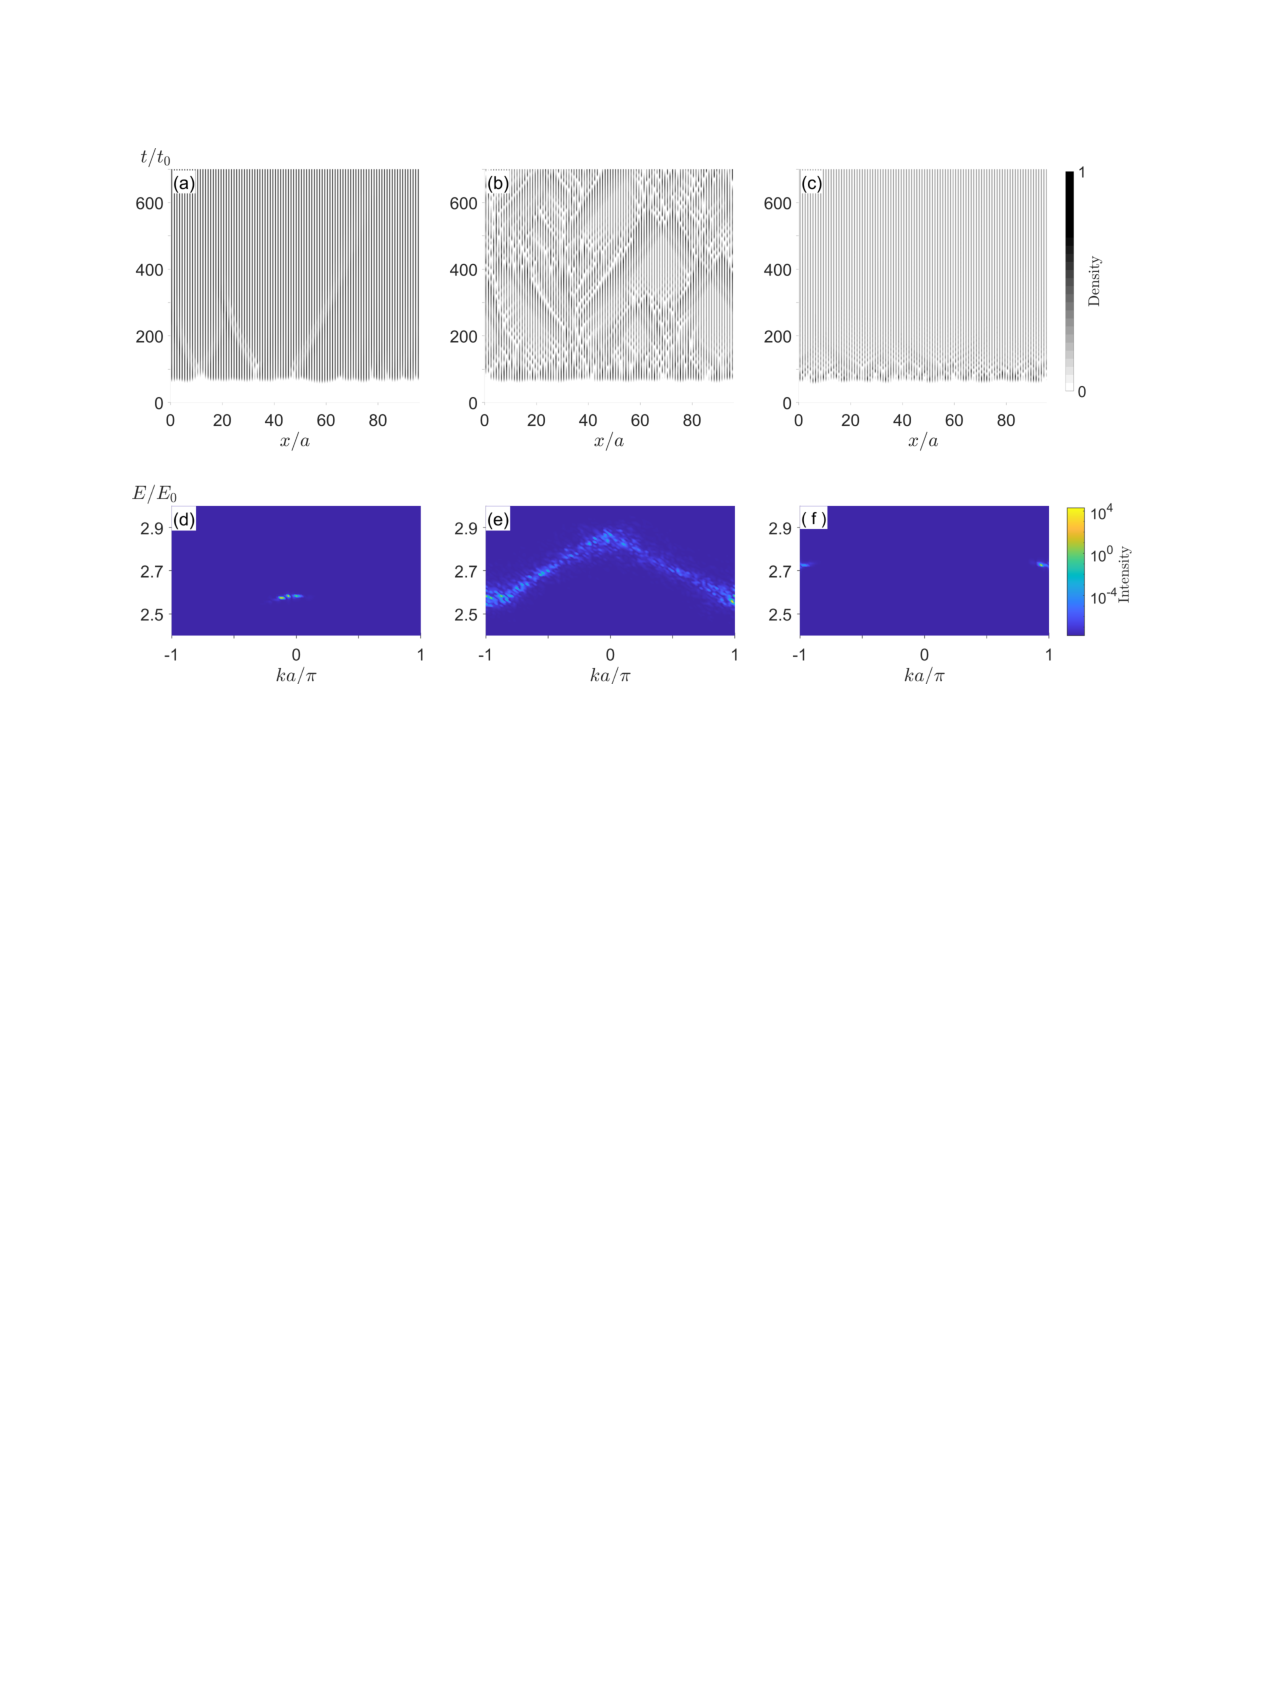
\includegraphics[width=0.85\textwidth]{Fig/Ch4/fig2.pdf}
\caption[Spatiotemporal patterns of the condensate density for the $\Lambda\Lambda$ case]{(a--c) Spatiotemporal patterns of condensate density $|\psi(x,t)|^2$, and (d--f) corresponding intensity $|\psi(k,E)|^2$ for the $\Lambda\Lambda$ case. The dimensionless interaction constant ($\alpha/\beta$) is equal to $0$, $2$, and $6$ in left, middle, and right panels, respectively. Time is measured in units of $t_0 \equiv \hbar/E_0$. The figure is taken from~\cite{Yoon:2019aa}.}
\label{CH4_fig:2-1}
\end{figure}

In what follows, we will consider the formation of the polariton condensate to be slightly above the threshold, when the losses in the system, as governed by the parameter $\Gamma$, are sufficient to make the first band the only one that possesses a positive imaginary part of the eigenvalue.
Thus, the particles are expected to condense into this band.
The complex potential in Fig.~\ref{CH4_fig:1-1} is then set by these two approaches:
(i) detuning the width and depth of the well to get ground state dispersion in the $\Lambda\Lambda$ (or VV) case, and (ii) changing the magnitude of the overall shift of the imaginary part to make the first band the only one with a positive imaginary part of the eigenvalue.
We also consider the first band to be well separated from the other bands, thus disregarding transitions between bands.

%
% ----------------------------
%
\subsection{Spatiotemporal dynamics of the condensate}

\begin{figure}[ht]
\centering
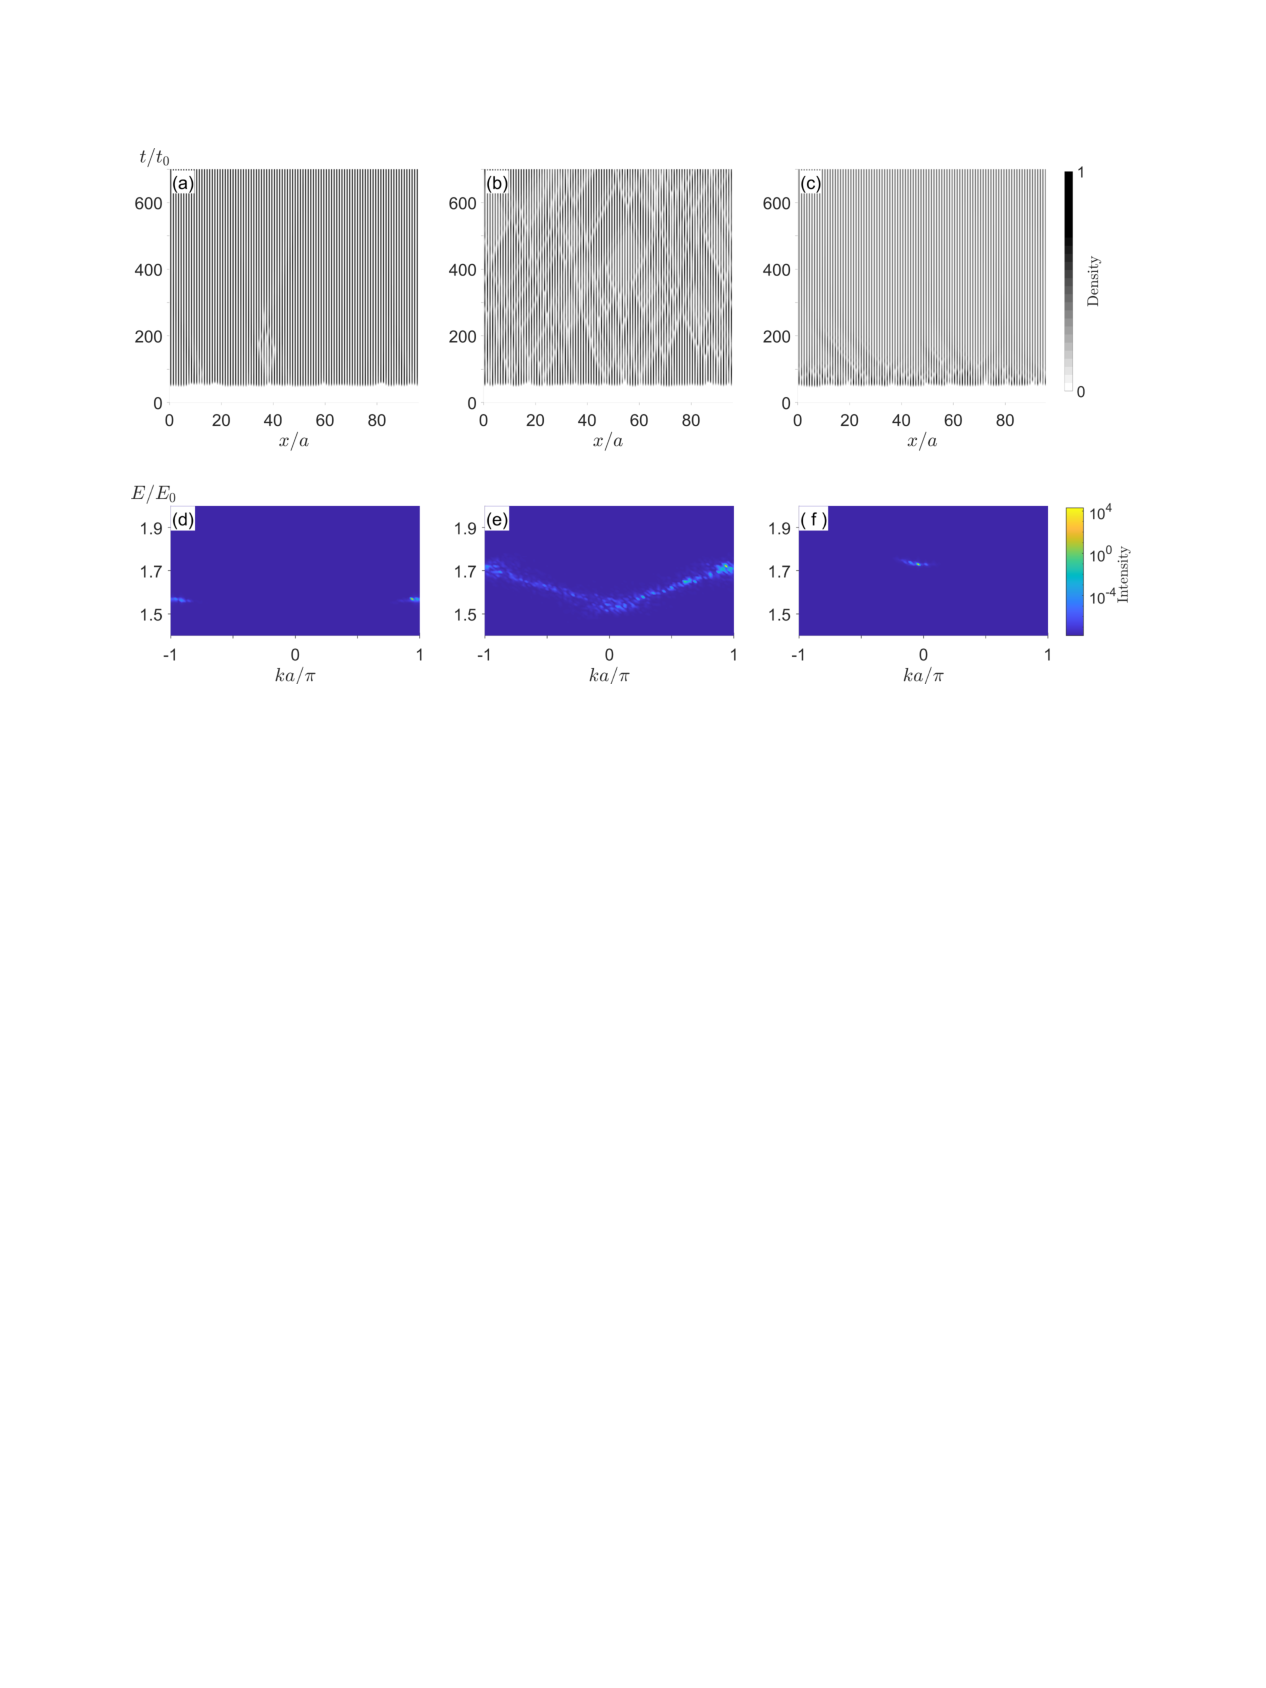
\includegraphics[width=0.85\textwidth]{Fig/Ch4/fig3.pdf}
\caption[Spatiotemporal patterns of the condensate density for the VV case]{(a--c) Spatiotemporal patterns of condensate density $|\psi(x,t)|^2$, and (d--f) corresponding intensity $|\psi(k,E)|^2$ (d, e, f) for the VV case. The dimensionless interaction constant ($\alpha/\beta$) is equal to $0$, $0.65$, and $2$ in left, middle, and right panels, respectively. The figure is taken from~\cite{Yoon:2019aa}.
}
\label{CH4_fig:2-2}
\end{figure}

For the non-interacting case, i.e. $\alpha = 0$ in Eq.~\eqref{eq:CH4_GPeq}, one expects to obtain the condensate in the state with the maximum gain.
Then the number of particles reaches its maximum in this state and can be stabilized by finite gain-dissipation parameter $\beta$.
Therefore, we can expect $0$-state condensation in the $\Lambda\Lambda$ and V$\Lambda$ cases, and $\pi$-state condensation in the $\Lambda$V and VV cases.
% Numerical solutions of Eq.~\eqref{eq:CH4_GPeq} show that this scenario remains valid even in the presence of strong repulsion between polaritons in the V$\Lambda$ and $\Lambda$V cases.
By checking the numerical simulations of Eq.~\eqref{eq:CH4_GPeq}, we can show that in the V$\Lambda$ and $\Lambda$V cases, this scenario of condensation persists even in the presence of strong repulsive polariton--polariton interaction.
However, the polariton--polariton interaction has a dramatic effect on the condensate loaded in the $\Lambda\Lambda$ and VV cases, leading to a fundamental reconstruction of the condensate state by increasing interactions.
Therefore, we will mostly concentrate on the VV and $\Lambda\Lambda$ configurations.

In Figs.~\ref{CH4_fig:2-1} and~\ref{CH4_fig:2-2}, we show the spatiotemporal dynamics of the condensate for the $\Lambda\Lambda$ and VV cases, respectively.
The upper rows of these figures show the spatiotemporal patterns of the condensate density, $|\psi(x,t)|^2$, and the lower ones show the polariton emission intensities, $|\psi(k,E)|^2$, for a small initial random seed of noise.
We calculated 50 trajectories and checked that different small initial random seeds give qualitatively similar pictures.
In the density plots, shown in the panels (a), (b), and (c) in both figures, the local maxima of the condensate density (dark black vertical lines along the time axis) are at the centers of the wells of the real potential $V_R$, where the maximal gain is attained [see also Fig.~\ref{CH4_fig:4}(a,b)].

From left to right in Figs.~\ref{CH4_fig:2-1} and \ref{CH4_fig:2-2}, the dimensionless parameter $\alpha/\beta$ increases and we observe considerable changes in the spatiotemporal density patterns and condensation states.
When $\alpha/\beta=0$, the condensate is formed in the state with the maximum gain: the $0$-state in the $\Lambda \Lambda$ case and the $\pi$-state in the VV case.
Defects appearing at the early stage of evolution dissipate away at later times.
When $\alpha/\beta$ takes an intermediate value, polaritons no longer accumulate in the state with a well-defined wave vector, but rather they distribute along the whole band.
As one can see from the corresponding panels [Figs.~\ref{CH4_fig:2-1}(b) and~\ref{CH4_fig:2-2}(b)], strong spatiotemporal chaos is present in this case.
Surprisingly, with further increase of the $\alpha/\beta$ ratio, well-defined condensation takes place again, but now the condensate is formed at the minimum of the dispersion, i.e. in the state with the smallest gain; this corresponds to the $\pi$-state in the $\Lambda \Lambda$ case and the $0$-state in the VV case.
This result is in contrast with the one obtained in the zero-interaction regime.
It should be noted that the $\pi$-state in our system is different from the one discussed in~\cite{Lai:2007aa}, where it corresponded to the minimum of the second band.

The density patterns presented in Figs.~\ref{CH4_fig:2-1}(c) and~\ref{CH4_fig:2-2}(c) resemble those of the spatiotemporal intermittency in the 1D complex Ginzburg--Landau equation (CGLE)~\cite{Chate:1994aa,Melo:1993aa,Hecke:1998aa},
which is
%
\begin{equation}\label{CH4_eq:NLSE}
\mi \partial_t A = \mi A + (c_1+ \mi )\partial_x^2 A + (c_3 - \mi)|A|^2 A \ .
\end{equation}
%
The nonlinear term here takes the same form as in Eq.~\eqref{eq:CH4_GPeq} and the linear terms for $c_1>0$ correspond to the complex-valued energy dispersion of the $\Lambda \Lambda$ case, even though the dispersion in Fig.~\ref{CH4_fig:1-1} is not a quadratic but a periodic function.
The parameters $c_1$ and $c_3$ play similar roles as ${\Delta}E_R/{\Delta}E_I$ and $\alpha/\beta$ in our system, respectively.
However, the shapes of the real and imaginary parts of the dispersion in Fig.~\ref{CH4_fig:1-1} are not exactly proportional to each other, and the \textit{continuous} translation symmetry of the CGLE is reduced to a \textit{discrete lattice} translation symmetry due to the periodic potential.

Another important difference is that even though the offset term $\mi A$ in Eq.~\eqref{CH4_eq:NLSE} admits only a restricted range of wave numbers ($-1<k<1$) to have a positive gain with a maximum at $k=0$, the edge points $k=\pm 1$ have zero gain, and therefore the condensate cannot be formed at the edge.
Instead, the polariton system is characterized by the edge points of the first Brillouin zone $k = \pm \pi/a$ with finite gain and the singularity in the density of states.
It is this feature that allows the formation of the polariton condensate at the edge.

In the system described by the CGLE, the spatiotemporal intermittent phase appears in the transition from a plain-wave state to a turbulent (chaotic) state~\cite{Chate:1994aa}.
In our case, the phase landscape is different: the spatiotemporal intermittency appears in the transistion from a $0$-state Bloch wave to a $\pi$-state Bloch-wave.
Nonetheless, the spatiotemporal intermittency pattern is quite similar to the conventional one.
We note that the intermittency phase exhibits some features of deterministic chaos within a single trajectory.
% A definite conclusion requires the study of the Lyapunov exponents, which is beyond the scope of this paper.
Similar intermittent polariton states have recently been reported in spontaneously-formed periodic structures under resonant driving~\cite{Gavrilov:2018aa}.

\begin{figure}[ht]
\centering
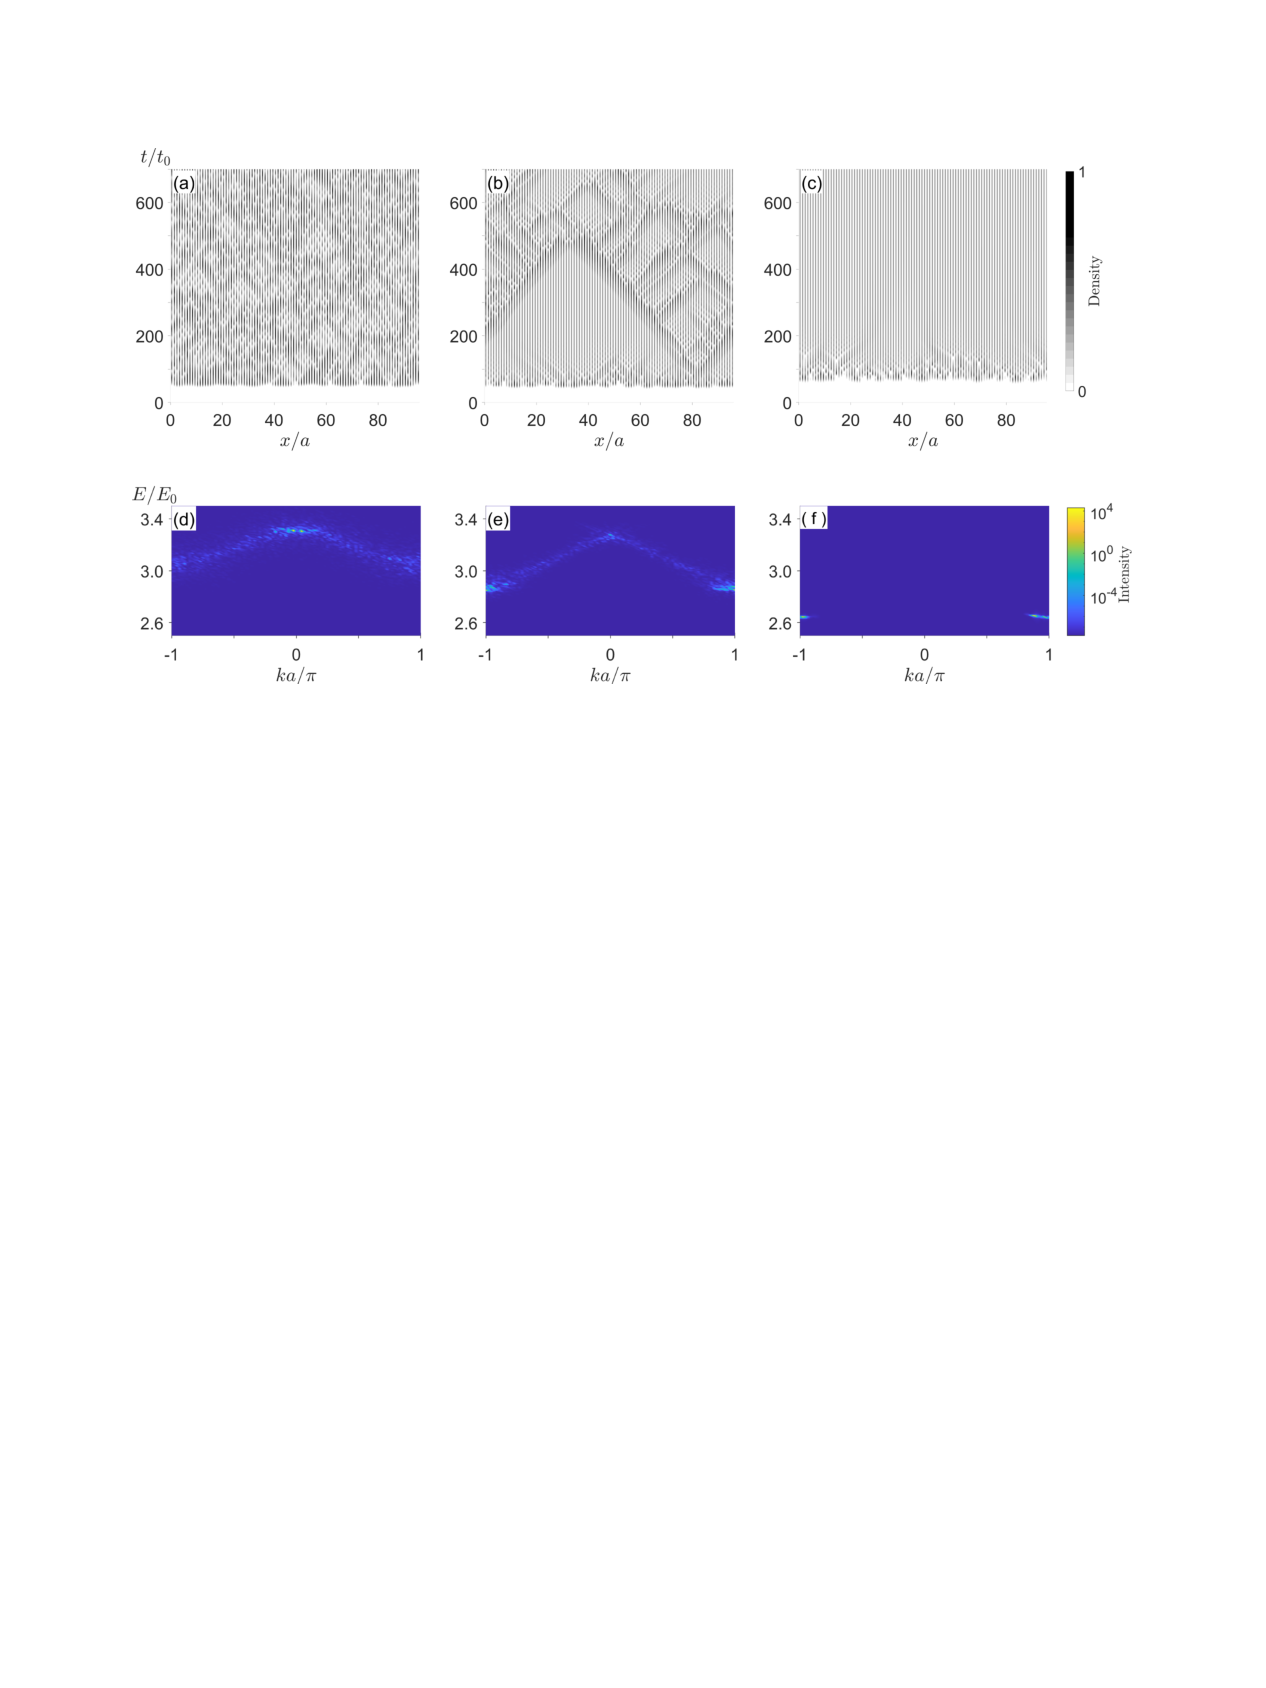
\includegraphics[width=0.85\textwidth]{Fig/Ch4/fig4.pdf}
\caption[Comparing spatiotemporal patterns with fixed nonlinearity]{(a--c) Spatiotemporal patterns of condensate density $|\psi(x,t)|^2$, and (d--f) corresponding intensity $|\psi(k,E)|^2$ for the $\Lambda\Lambda$ case with $\alpha/\beta = 4$ fixed. From left to right: the ratios of the real and imaginary parts of the energy bandwidths are ${\Delta}E_R/{\Delta}E_I \approx 1$, $2$, and $4$; $W = 3.82~U$, $3.43~U$, and $3.18~U$ with $U=14(\hbar^2/m^* a^2)$; and $\Delta E_R \approx  0.107~E_0$, $0.164~E_0$, and $0.201~E_0$ with $E_0=\pi^2\hbar^2/2m^*a^2$, respectively. The figure is taken from~\cite{Yoon:2019aa}.}
\label{CH4_fig:3-1}
\end{figure}

The crossover from spatiotemporal intermittent dynamics to the $\pi$-condensate in the $\Lambda\Lambda$ case (or to the $0$-condensate in the VV case) is not always possible.
The formation of a new condensate phase depends not only on the polariton interaction strength $\alpha/\beta$, as has been discussed above, but also on the ratio ${\Delta}E_R/{\Delta}E_I$.
Figure~\ref{CH4_fig:3-1} demonstrates (for the $\Lambda\Lambda$ case) that a sufficiently large value of the ratio ${\Delta}E_R/{\Delta}E_I$ is required to reach a $\pi$-state from the mixture of spatiotemporal intermittency states.

%
% ----------------------------
%
\subsection{Spatiotemporal intermittency}
The transition from a regular/laminar state to an irregular/turbulent state via spatiotemporal intermittency has been suggested to be related to the directed-percolation process~\cite{Pomeau:1986aa}.
Following directed percolation studies, spatial intermittency can be quantified by measuring the distribution of the lengths of laminar domains, and this is expected to reveal a power-law behavior at the threshold of spatiotemporal intermittency~\cite{Chate:1987aa, Chate:1994aa}.

The spatiotemporal pattern we observe is not exactly the same as in conventional spatiotemporal intermittency~\cite{Pomeau:1986aa}, because, in our system, the intermittent pattern appears halfway between two ordered phases ($0$- and $\pi$-phases).
On both sides of the intermittency domain, there is only one stable condensate state.
Inside the intermittency domain, both $0$- and $\pi$-phases of the condensate are stable, but they possess different basins of attraction.
The basin of attraction of the new phase grows with increasing polariton--polariton interaction, while the basin of attraction of the old phase shrinks down.
Near the boundary of the intermittency domain, a phase with a smaller basin of attraction is created by the propagating solitons, which have the form of small domains of this less-probable phase.
%More detailed analysis involves studying the sizes of basins of attraction and the Lyapunov exponents of the two phases in question and it is beyond the scope of this paper.

%
%
%
\begin{figure}[ht]
\centering
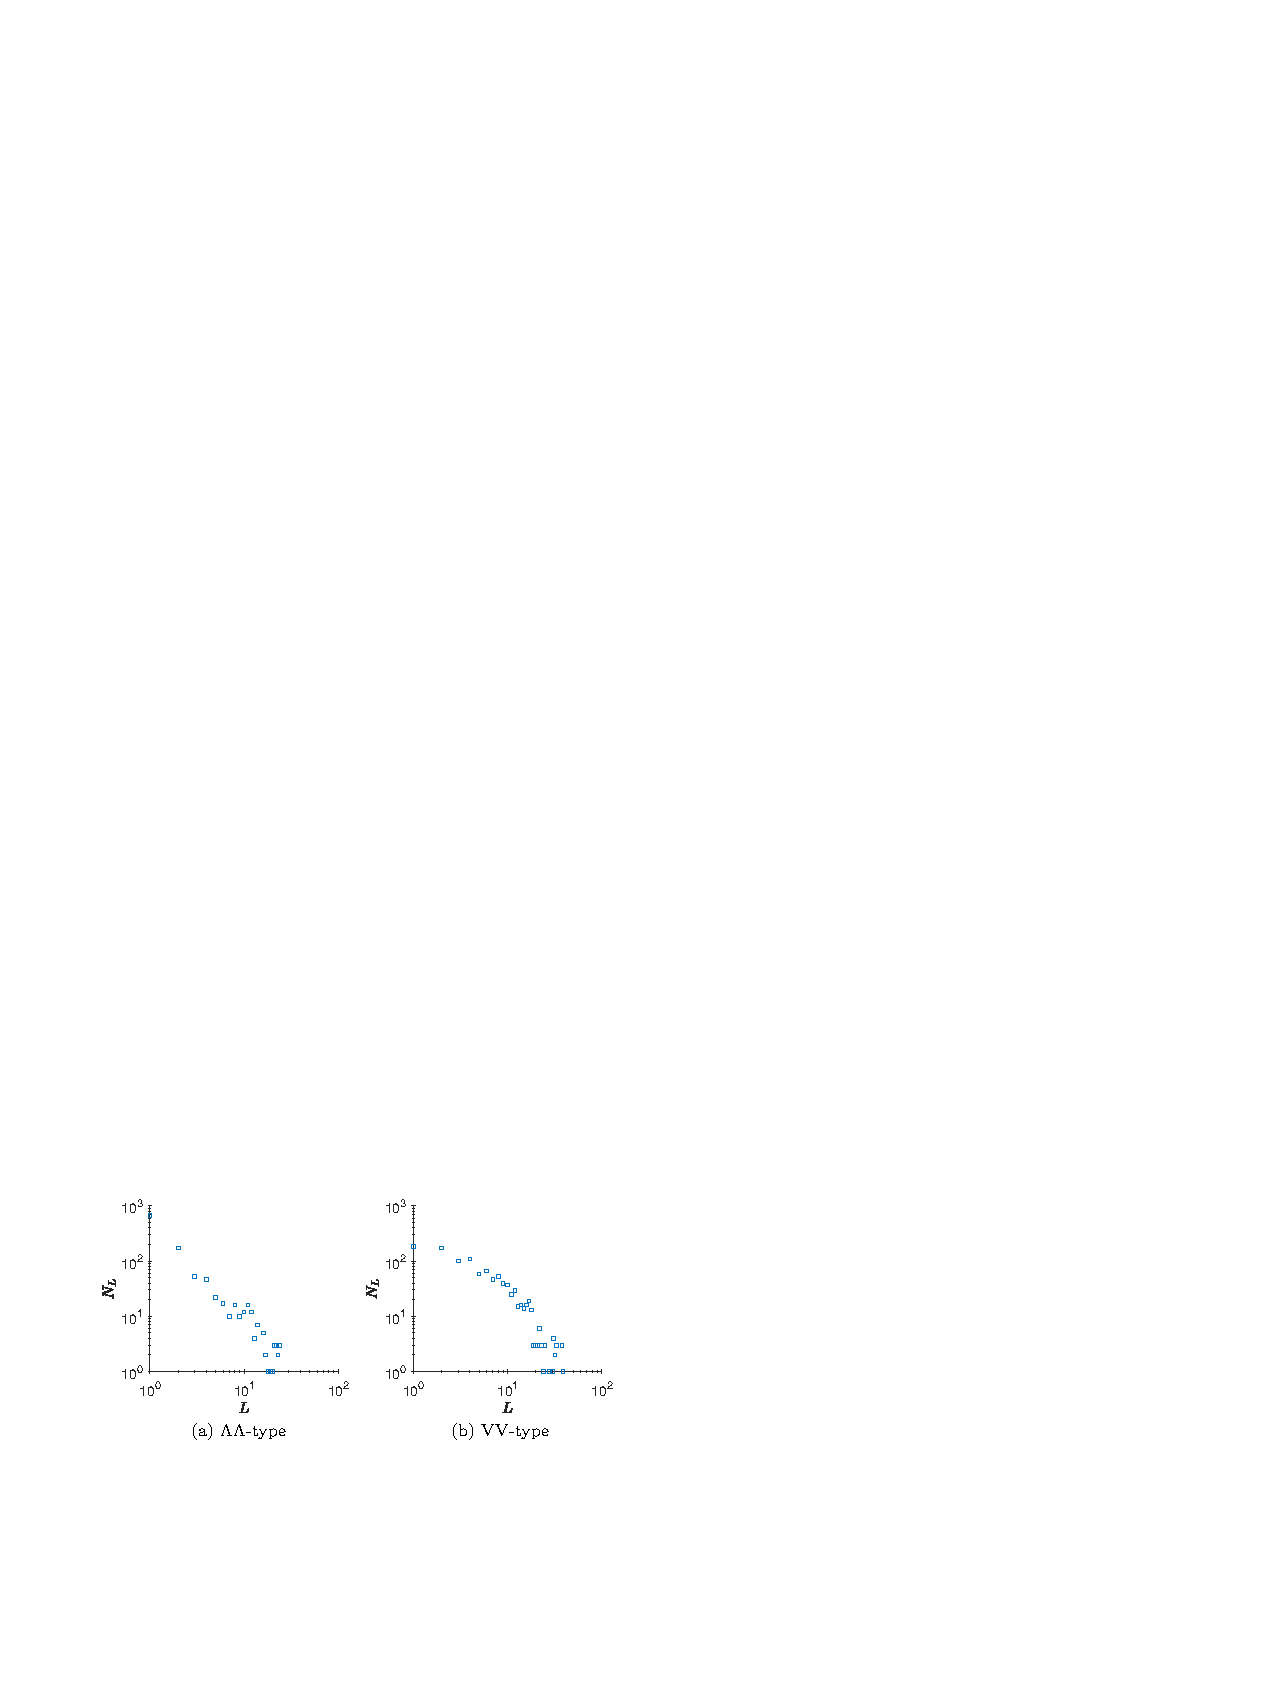
\includegraphics[width=0.75\textwidth]{Fig/Ch4/fig5.pdf}
\caption[Distributions of the number of defect domains]{Distributions of the number of defect domains ($N_L$) for the spatiotemporal patterns presented in (left) Fig.~\ref{CH4_fig:2-1}(b), and (right) Fig.~\ref{CH4_fig:2-2}(b).
%The parameters of the potential and $\alpha/\beta$ are also taken as in Fig.~2(b) for panel (a) here and as in Fig.~3(b) for panel (b).
$N_L$ is sampled from $t/t_0=200$ to $t/t_0=700$ with a time interval of $t/t_0=5$.
%for the $\Lambda\Lambda$ case (left panel) and $VV$ case (right panel).
Both horizontal and vertical axes are in log scale. The figure is taken from~\cite{Yoon:2019aa}.}
\label{CH4_fig:1}
\end{figure}
%
%

However, the spatiotemporal pattern in our case is quite similar to the one appearing in the transition to turbulence.
We also consider the distribution of lengths of the defect domains, which represent domains of dark solitons in the $\Lambda \Lambda$ case and domains of the absence of dark solitons in the VV case.
Figure~\ref{CH4_fig:1} shows the distributions of $N_L$ (number of defect domains of length $L$).
%
Here $N_L$ is sampled at $t/t_0 = 200\to 700$ with a time interval of $5$. We have checked that the linearly declining behavior (in log-log scale) is insensitive to the choice of smaller time intervals.
We indeed observe a behavior close to power-law, which is the fingerprint of spatiotemporal intermittency.

%
% ---------------------------------
%
\subsection{Soliton dynamics}
%
%
%
\begin{figure}[ht]
\centering
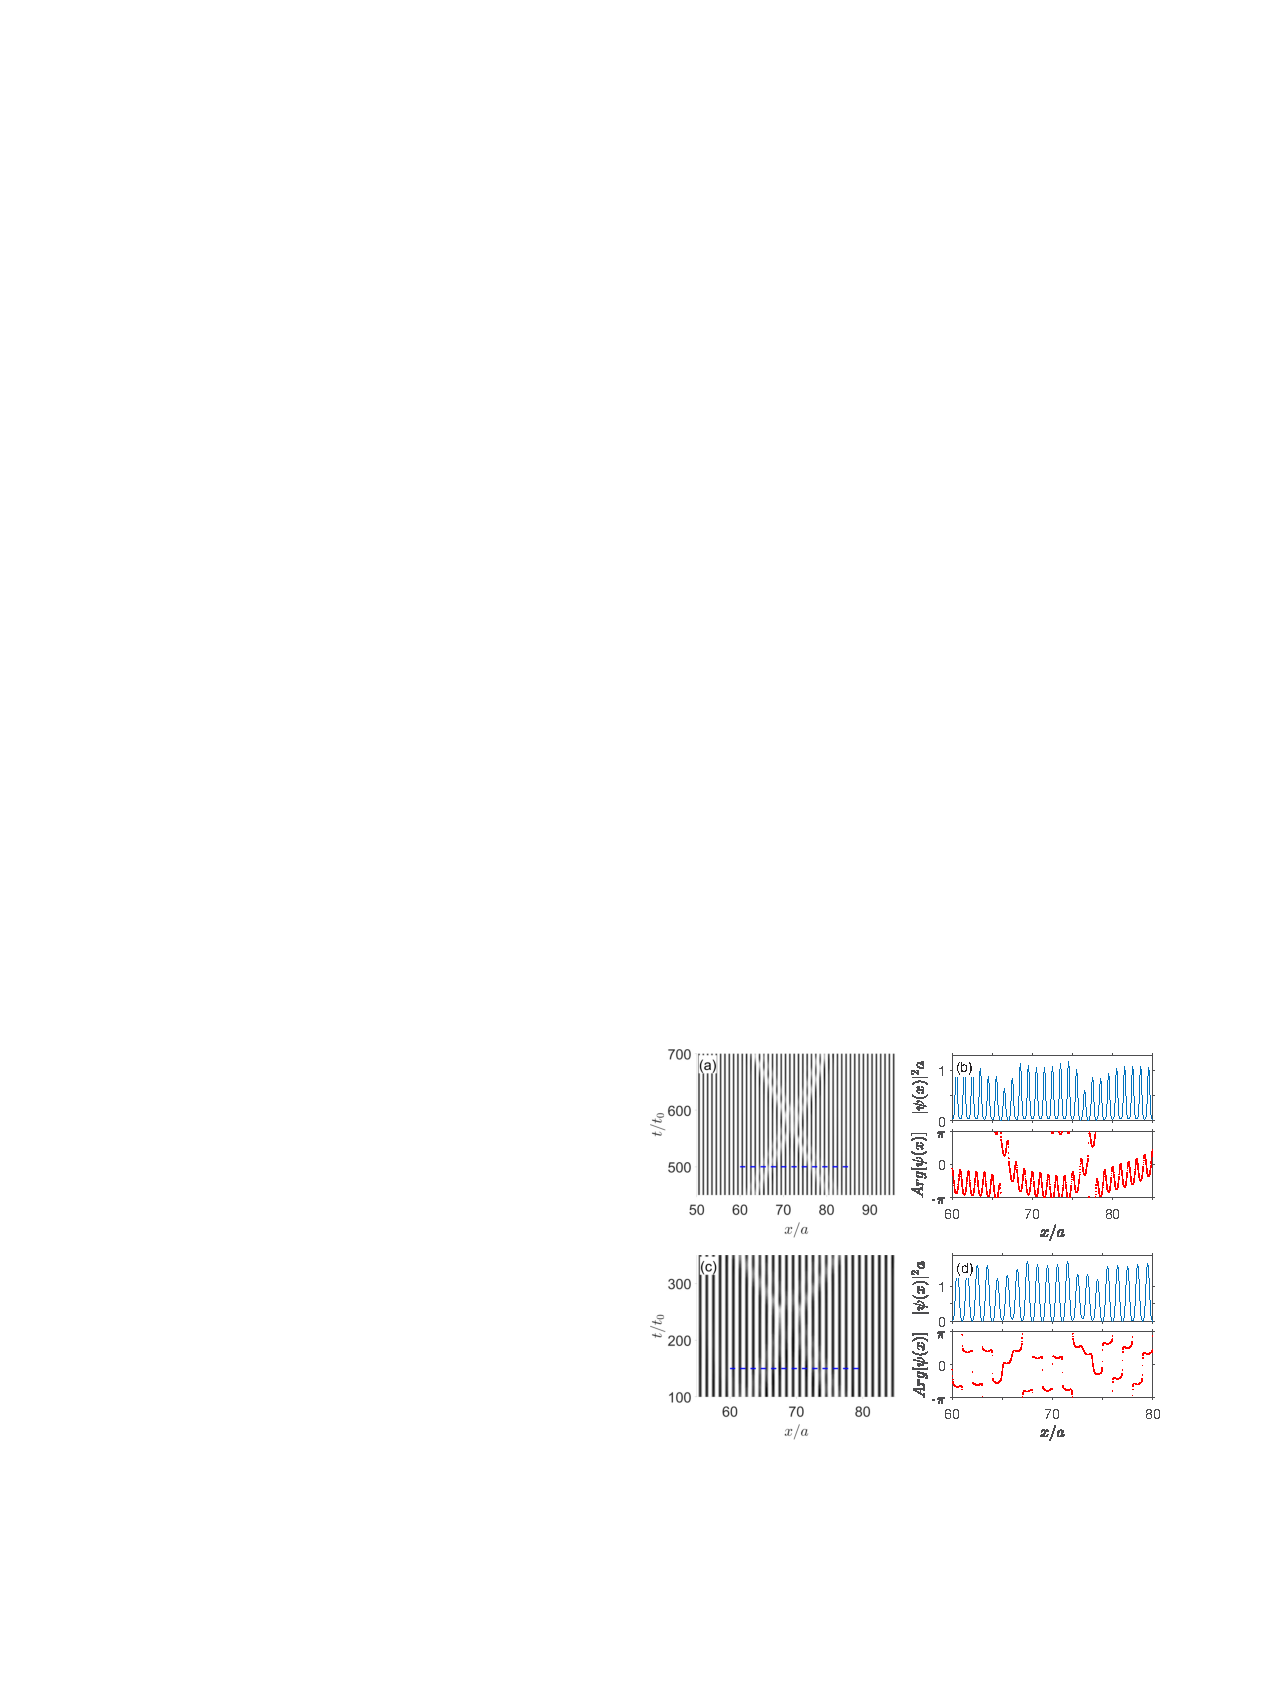
\includegraphics[width=0.85\textwidth]{Fig/Ch4/fig6.pdf}
\caption[Propagation and collision of solitons]{Propagation and collision of a pair of solitons in (a,b) the $\Lambda\Lambda$ case and (c,d) the VV case, for $\alpha/\beta=0.4$ when the number of solitons is small. (b,d) Upscaled particle density profiles and the phases of the wave functions just before the collisions marked by the thick dashed blue lines in (a,c), respectively. The figure is taken from~\cite{Yoon:2019aa}.}
\label{CH4_fig:4}
\end{figure}
%
%
%

At weak polariton--polariton interaction, the long-range order of the $0$-condensate in the $\Lambda\Lambda$ case and the $\pi$-condensate in the VV case is destroyed by the formation of propagating defects.
Each defect extends only over a few lattice constants, and they are characterized by the suppression of condensate occupation and by the phase slips.

As an example, Fig.~\ref{CH4_fig:4} shows the collision events of a pair of such defects propagating towards each other.
Individual collisions are seen only for weakly interacting polaritons when the concentration of defects is small.
Each defect is characterized by a depletion of particle density together with an abrupt change in the phase of the wave function at two edge points of the defect, where the phase change is about $\pi$ in the $\Lambda\Lambda$ case and smooth in the VV case.
The fact that the defects maintain their properties after the collision indicates that they can also be considered as dark solitons.
We note, however, that these solitons differ from the Bekki--Nozaki hole solutions of the CGLE~\cite{Bekki:1985aa} and the dissipative Gross--Pitaevskii equation for polariton mean field~\cite{Xue:2014aa}.
In our case, solitons represent the building blocks of a new condensate phase.

Soliton density increases with $\alpha/\beta$, and some of them attach to each other to form wide soliton domains, which one can see in Figs.~\ref{CH4_fig:2-1}(b) and~\ref{CH4_fig:2-2}(b).
In the $\Lambda\Lambda$ case, with a further increase of polariton--polariton interaction and for a sufficiently large ${\Delta}E_R/{\Delta}E_I$ ratio, a complete array of dark solitons is formed as in Fig.~\ref{CH4_fig:2-1}(c).
The wave function phase changes by $\pi$ per every lattice constant and the quasi-long-range order appears again, manifesting the formation of a $\pi$-condensate phase.

%
% ----------------------------------
%
\subsection{Summary}
We have shown that interacting exciton-polaritons loaded into a one-dimensional microcavity with a periodic potential and periodic distribution of losses can condense into nontrivial states, where losses are not minimized but rather maximized.
Under certain conditions, polaritons can form a space-time intermittency phase, which separates two condensate phases with minimal and maximal losses.
The reconstruction of the condensate wave function takes place by a proliferation of dark solitons along the periodic structure.
The nuclei of the new condensate phase, which are characterized by the maximization of losses, are formed with increasing polariton--polariton interaction, and they can be seen as a result of dark solitons gluing  together.
